\documentclass[12pt]{article}

\usepackage[utf8]{inputenc} 
\usepackage[T1]{fontenc}   
\usepackage{hyperref}       
\usepackage{url}           
\usepackage{booktabs}       
\usepackage{amsfonts}       
\usepackage{amsmath}  
\usepackage{nicefrac}      
\usepackage{microtype}      
\usepackage{lipsum}
\usepackage{graphicx}
\usepackage{float}
\usepackage{indentfirst}
\usepackage{setspace}
\usepackage{geometry}
\usepackage{caption}
\usepackage{subcaption}
\usepackage{listings}
\usepackage{pgfplots}
\usepackage{adjustbox}
\geometry{
    a4paper,
    left=25mm,
    right=25mm,
    top=25mm,
    bottom=25mm
}

\begin{document}
\author{Jędrzej Szor 239716}
\title{\text{Obliczenia ewolucyjne}\\\textbf{Implementacja algorytmu BOA z wzorcem}}
\maketitle

\section{Opis zaproponowanej wersji algorytmu BOA}
Zaimplementowana przeze mnie wersja algorytmu BOA bazuje na dokumencie zamieszczonym na wikampie. Na jedną iterację składa się obliczenie zapachu dla każdego motyla w roju, wybranie najlepszego osobnika oraz obliczenie nowych koordynatów dla każdego motyla. Zapach oblicza się na podstawie poniższych wzorów:
\begin{equation}
    f = cI^a
\end{equation}
\begin{equation}
    I = \frac{1}{F}
\end{equation}
gdzie $F$ jest wartością funkcji dla aktualnych współrzędnych motyla.\\
Zastosowany sposób obliczania zapachu podstawowego $I$ pozwala osiągnąć minimum globalne będące $\geq 0$. W przypadku globalnego minimum $\le 0$ pojawiają się liczby zespolone, w które się nie zagłębiałem.
\begin{figure}[H]
    \centering
    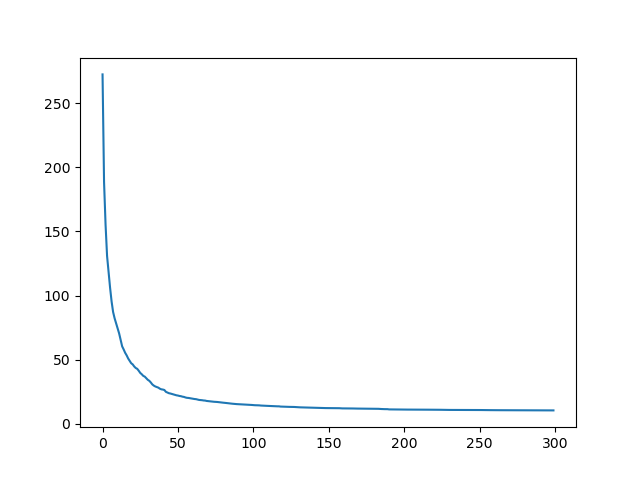
\includegraphics[width=10cm]{plots/up10.png}
    \caption{Wykres najlepszych wartości dla funkcji sfery podniesionej o 10.}
\end{figure}

Jeśli chodzi o wzorce, zastosowałem metodę genetyczną opisaną w treści zadania. W pierwszej kolejności wybierany jest najlepszy osobnik z puli wzorców a następnie każdy osobnik jest z nim krzyżowany w przypakowo ustalonej konfiguracji procentowej. Następnie każda ze współrzędnych każdego osobnika może zostać zmutowana z 5\% prawdopodobieństwem. Na końcu następuje walidacja, która upewnia się że żaden wzorzec nie jest gorszy niż był. Wzorce generowane są przed krokiem algorytmu BOA i wliczane są do puli motyli, czyli obliczany jest dla nich zapach i brane są pod uwagę podczas wyboru najlepszego osobnika. 


\section{Wyniki}
Poniżej zaprezentowane są wyniki przebiegu algorytmu dla różnych konfiguracji. Wykresy zostały sporządzone na podstawie 30 przebiegów algorytmów po 300 iteracji dla dziedzin przewidzianych w dokumencie z opisami funkcji. Zastosowane stałe parametry algorytmu BOA to c = 0.01, a = 0.2, p = 0.8.

\subsection{Wyniki dla funkcji sfery}
\begin{figure}[H]
    \centering
    \begin{subfigure}{0.32\textwidth}
        \centering
        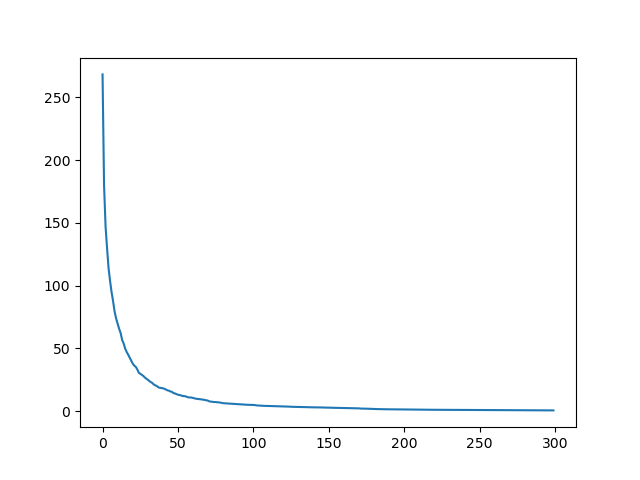
\includegraphics[width=\linewidth]{plots/s1.png}
        \caption{Populacja = 20, min = 0.2, czas wykonywania 11.04s}
    \end{subfigure}
    \begin{subfigure}{0.32\textwidth}
        \centering
        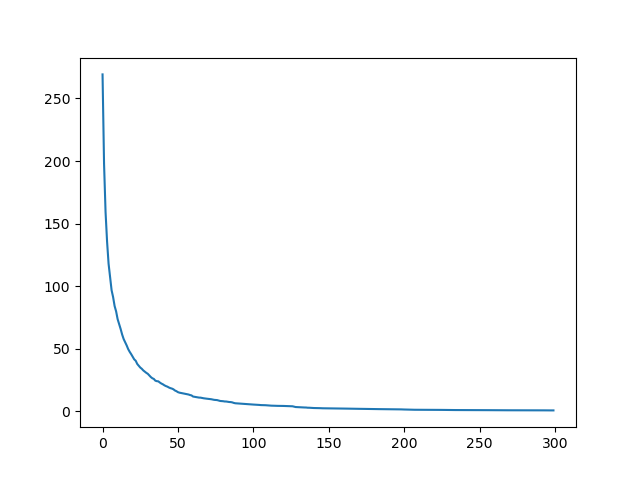
\includegraphics[width=\linewidth]{plots/s2.png}
        \caption{Populacja = 30, min = 0.24, czas wykonywania 12.77s}
    \end{subfigure}
    \begin{subfigure}{0.32\textwidth}
        \centering
        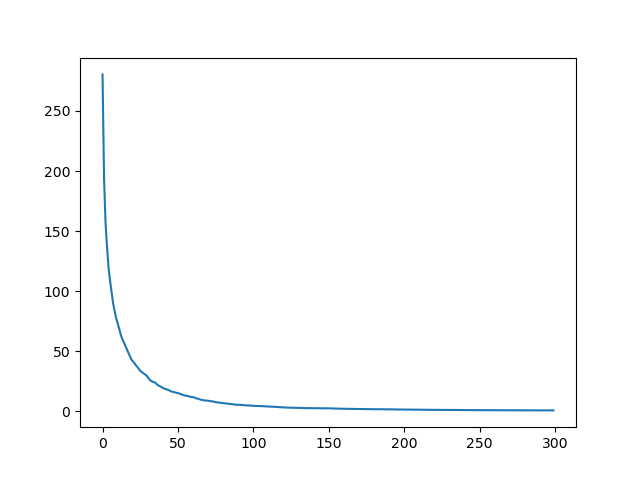
\includegraphics[width=\linewidth]{plots/s3.png}
        \caption{Populacja = 50, min = 0.13, czas wykonywania 15.91s}
    \end{subfigure}
    \caption{Wyniki dla zmiennej liczby populacji. Populacja wzorców = 10}
\end{figure}

\begin{figure}[H]
    \centering
    \begin{subfigure}{0.32\textwidth}
        \centering
        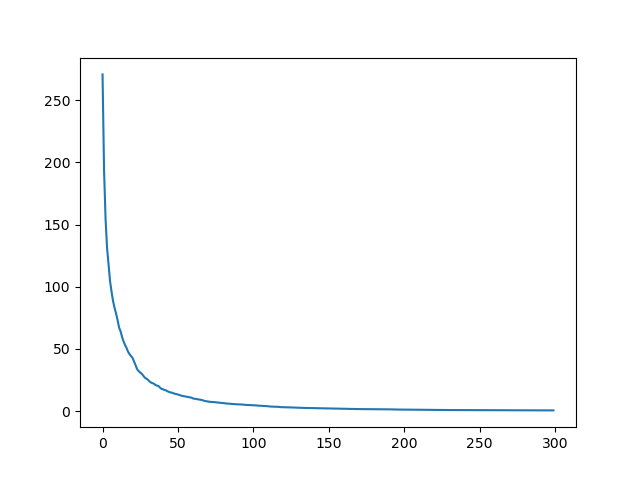
\includegraphics[width=\linewidth]{plots/s4.png}
        \caption{Liczba wymiarów = 20, min = 0.16, czas wykonywania 14.41s}
    \end{subfigure}
    \begin{subfigure}{0.32\textwidth}
        \centering
        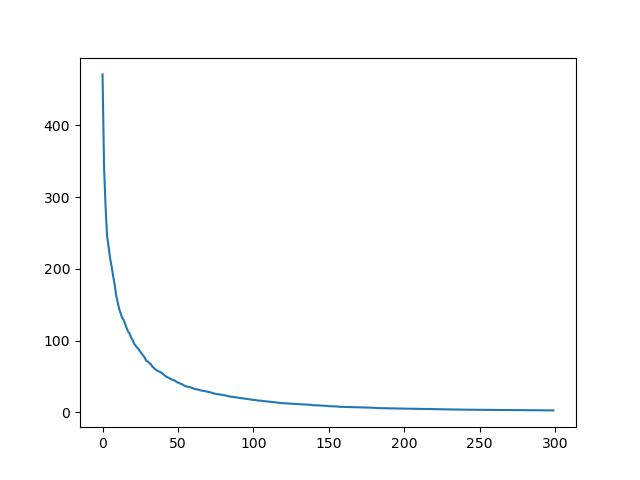
\includegraphics[width=\linewidth]{plots/s5.png}
        \caption{Liczba wymiarów = 30, min = 1.36, czas wykonywania 19.86s}
    \end{subfigure}
    \caption{Wyniki dla zmiennej liczby wymiarów. Populacja wzorców = 10, liczba populacji = 40}
\end{figure}

\begin{figure}[H]
    \centering
    \begin{subfigure}{0.32\textwidth}
        \centering
        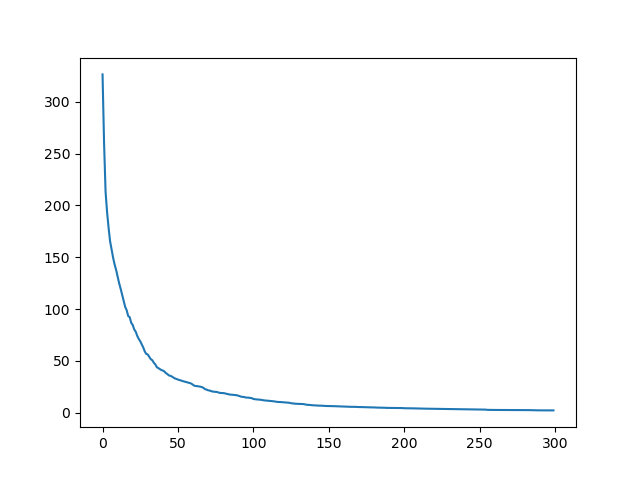
\includegraphics[width=\linewidth]{plots/s6.png}
        \caption{Populacja wzorców = 5, min = 0.96, czas wykonywania 10.52s}
    \end{subfigure}
    \begin{subfigure}{0.32\textwidth}
        \centering
        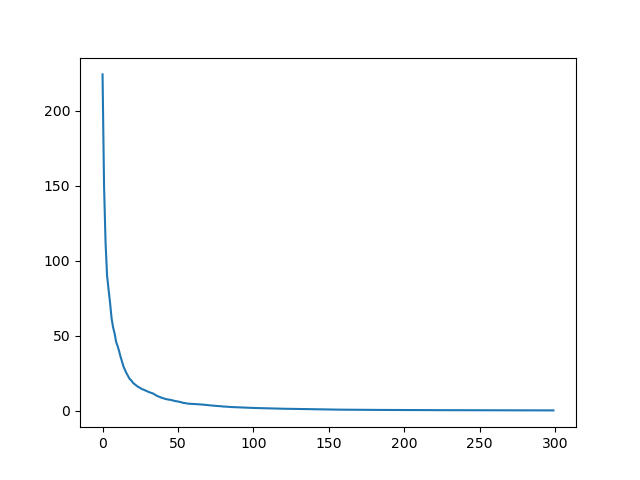
\includegraphics[width=\linewidth]{plots/s7.png}
        \caption{Populacja wzorców = 20, min = 0.05, czas wykonywania 21.81s}
    \end{subfigure}
    \begin{subfigure}{0.32\textwidth}
        \centering
        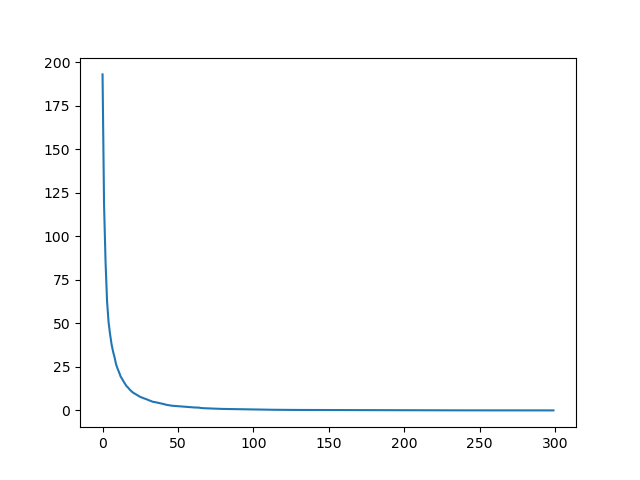
\includegraphics[width=\linewidth]{plots/s8.png}
        \caption{Populacja wzorców = 30, min = 0.04, czas wykonywania 29.02s}
    \end{subfigure}
    \caption{Wyniki dla zmiennej liczby populacji wzorców. Liczba populacji = 40}
\end{figure}


\subsection{Wyniki dla funkcji Corana}
\begin{figure}[H]
    \centering
    \begin{subfigure}{0.32\textwidth}
        \centering
        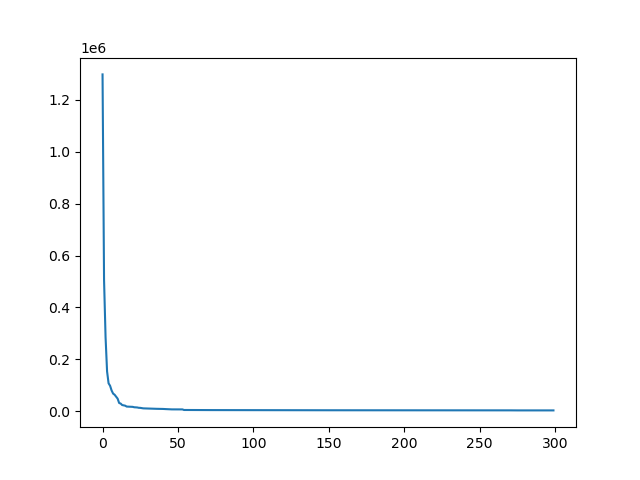
\includegraphics[width=\linewidth]{plots/c1.png}
        \caption{Populacja = 20, min = 0.0, czas wykonywania 21.67s}
    \end{subfigure}
    \begin{subfigure}{0.32\textwidth}
        \centering
        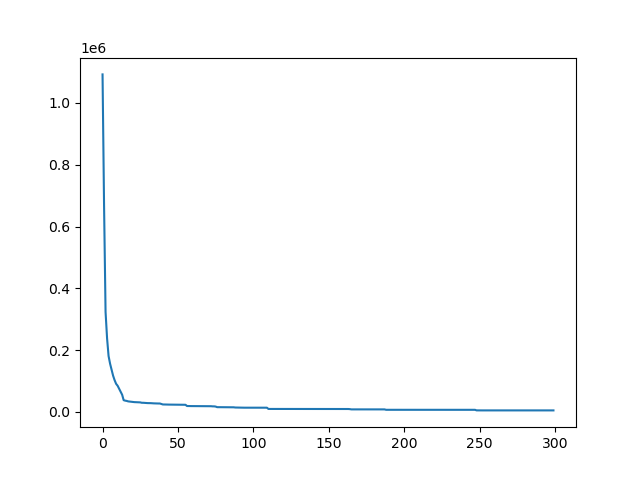
\includegraphics[width=\linewidth]{plots/c2.png}
        \caption{Populacja = 30, min = 0.003, czas wykonywania 24.74s}
    \end{subfigure}
    \begin{subfigure}{0.32\textwidth}
        \centering
        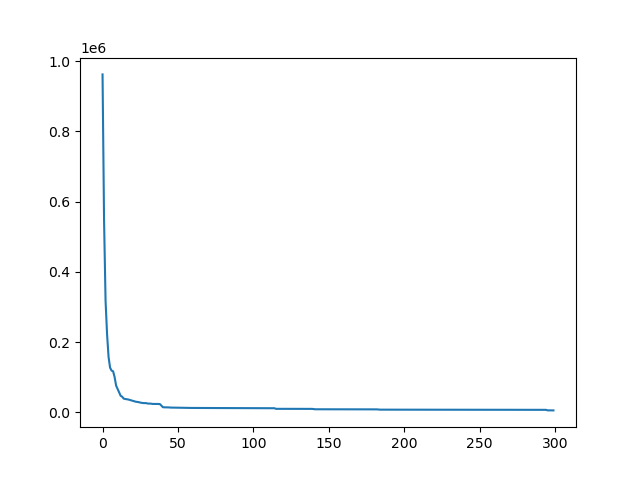
\includegraphics[width=\linewidth]{plots/c3.png}
        \caption{Populacja = 50, min = 0.03, czas wykonywania 29.33s}
    \end{subfigure}
    \caption{Wyniki dla zmiennej liczby populacji. Populacja wzoców = 10}
\end{figure}

\begin{figure}[H]
    \centering
    \begin{subfigure}{0.32\textwidth}
        \centering
        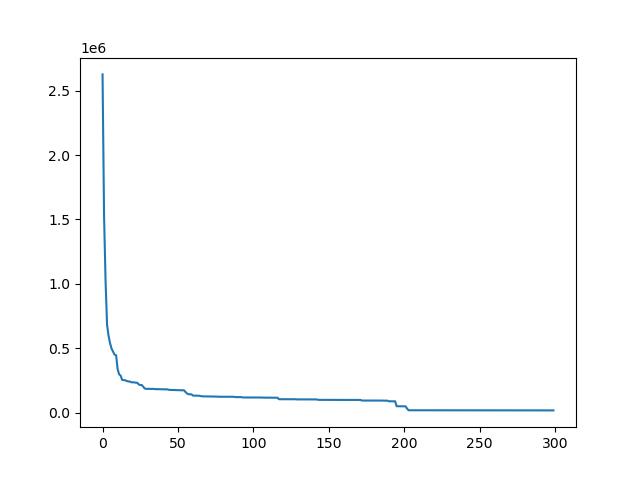
\includegraphics[width=\linewidth]{plots/c4.png}
        \caption{Populacja wzorców = 5, min = 5.70, czas wykonywania 19.10s}
    \end{subfigure}
    \begin{subfigure}{0.32\textwidth}
        \centering
        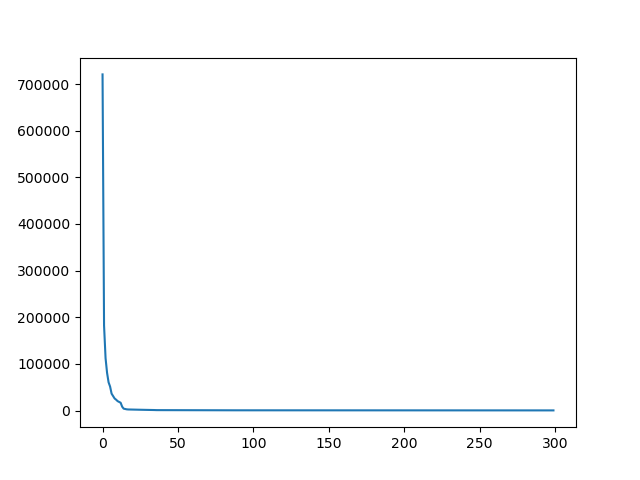
\includegraphics[width=\linewidth]{plots/c5.png}
        \caption{Populacja wzorców = 20, min = 0.03, czas wykonywania 42.77s}
    \end{subfigure}
    \begin{subfigure}{0.32\textwidth}
        \centering
        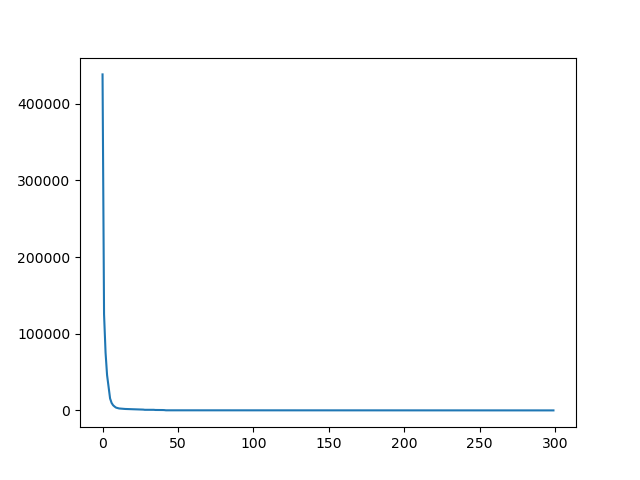
\includegraphics[width=\linewidth]{plots/c6.png}
        \caption{Populacja wzorców = 30, min = 0.0, czas wykonywania 58.19s}
    \end{subfigure}
    \caption{Wyniki dla zmiennej liczby populacji wzorców. Liczba populacji = 40}
\end{figure}


 
\section{Wnioski}
Algorytm BOA z wzorcem ma łagodniejszy przebieg niż zwykły algorytm BOA. Charakterystyka przebiegu jest dużo płynniejsza i nie ma poszarpanych krawędzi. Wzorce generowane metodą genetyczną prowadzą algorytm oraz poprawiają jego wiarygodność pozostawiając jednocześnie lekki obliczeniowo charakter i bardzo szybki czas wykonywania.

\end{document}